\chapter{Анализ механизмов движения мобильных плавающих роботов}\label{ch:ch1}

\section{Введение}\label{sec:ch1/sec1}

В последние десятилетия активно развивается область по разработке мобильных роботов. В настоящее время уделяется существенное внимание разработке автономных мобильных роботов, предназначенных для решения определенных задач в разных средах. Появляющиеся роботы охватывают различные среды: роботы, перемещающиеся по твердой поверхности \todo{вместо скобочек добавить ссылки} (автономные автомобили), роботы, перемещающиеся по воздуху (автономные коптеры, самолеты и т. д.), водные роботы, перемещающиеся по поверхности жидкости (автономные катера) и на глубине (автономные подводные аппараты). 

Развиваются области в создании роботов использующих как более традиционные способы перемещения, так и имеющие новые принципы приведения в движение. Отдельную область составляет исследование динамики водных роботов, имитирующих способы передвижения живых существ и роботов, не имеющих внешних подвижных элементов. Передвижение таких устройств реализуется за счет движения внутренних масс и вращения роторов. Такие «экзотические» транспортные средства могут применяться в специфических (критических) условиях, например в условиях космоса или на больших глубинах.

\section{Обзор способов перемещения роботов в жидкости}\label{sec:ch1/sec21}

Выделим существующие способы перемещения в жидкости:

\begin{enumerate}
	\item Перемещение за счет использования гребных винтов.
	\item Перемещение за счет изменения формы тела.
	\item Перемещение за счет использования реактивного привода.
	\item Перемещение за счет действия внутренних механизмов.
\end{enumerate}

Рассмотрим подробнее каждый из этих способов.

\subsection{Перемещение за счет использования гребных винтов}\label{sec:ch1/sec2}

В настоящее время для водных мобильных систем самым распространенным способом перемещния является перемещение с помощью винтов. Способ перемещения с помощью винтов называют традиционным способом. Аппараты, используемые гребные винты широко используются для мониторинга и проведения различных операций. В частности, для мониторинга подводного рельефа и подводной геологоразведки, мониторинга обшивок подводных конструкций, проведение ремонтных работ на больших глубинах и в условиях химического или радиационного загрязнения и т.д. 





\subsection{Перемещение за счет изменения формы тела}\label{sec:ch1/sec3}


\subsection{Перемещение за счет реактивной тяги}\label{sec:ch1/sec4}



\subsection{Перемещение за счет внутренних механизмов}\label{sec:ch1/sec5}

Для описания управляемого движения твердых тел в жидкости были предложены различные математические модели. Наиболее простые модели основаны построены в рамках теории идеальной жидкости и учитывают только эффект присоединенных масс. Однако такие существенно упрощенные модели позволяют обнаружить интересные динамические эффекты и закономерности, наблюдаемые в экспериментах. Например, в работах \cite{Kozlov_Ramodanov_PMM_2001, Kozlov_Onichenko} рассматривалось продвижение твердых тел в идеальной жидкости за счет подвижных внутренних масс. Было показано, что неограниченное продвижение оказывается возможным только при наличии анизотропии присоединенных масс. Идеи работ \cite{Kozlov_Ramodanov_PMM_2001, Kozlov_Onichenko} получили развитие в \cite{Vetchanin_Kilin_2016}, где рассматривалось движение эллиптического профиля, содержащего два эксцентрика, вращающихся в одинаковыми по модулю и противоположными по знаку скоростями. Было показано, что такая система движется в среднем прямолинейно. Данный факт подтверждается экспериментально, см. \cite{Klenov_Kilin_2016}. Также отметим работу \cite{Jing_Kanso_2013}, где рассматривалась задача устойчивости движения эллиптического профиля за счет вращательных колебаний. Трехмерные задачи управления и стабилизации движения эллипсоидов и винтовых тел рассматривались, например, в работах \cite{Borisov_et_al_2017, Vetchanin_Mamaev_2017, Vetchanin_et_al_2016, Woolsey_Leonard_1999}.

Модель схода вихрей позволяет описать самопродвижение тела за счет колебаний внутреннего ротора, наблюдаемое в экспериментах \cite{Tallapragada_2015, Pollard_Tallapragada_2019}. Однако, следует отметить, что сход каждого вихря приводит к увеличению размерности фазового пространства системы, что влечет определенные вычислительные трудности. Альтернативой описанной модели являются конечномерные математические модели, учитывающие вязкое трение и изменение циркуляции. Например, в работе \cite{Borisov_et_al_2018} рассматривалось плоскопараллельное движение эллиптического профиля за счет колеблющегося ротора при наличии периодически изменяющейся циркуляции и вязкого трения. Подобная модель для тела с острой кромкой и циркуляцией, изменяющейся согласно условию Кутты-Чаплыгина, была предложена в работе \cite{Mamaev_Vetchanin_2018} на основе результатов численных экспериментов, описанных в работе \cite{Mamaev_et_al_2018}. В работе \cite{Kilin_et_al_2018} была предложена модель движения робота с двумя эксцентриками, учитывающая помимо вязкого сопротивления, качку во время движения.

Отметим, что наиболее полное описание движения тел в жидкости может быть получено на основе совместного решения уравнений движения тела и уравнений Навье-Стокса, см., например, работы \cite{Childress_et_al_2011, Eldredge_2006, Vetchanin_et_al_2013}. Однако использование такого подхода затратно с вычислительной точки зрения при исследовании управляемого движения и построении гейтов. Поэтому моделирование с использованием уравнений Навье-Стокса целесообразно только при построении конечномерных моделей движения тел в жидкости, которые оказывают более удобными при анализе управляемого движения.




Рассмотрим более подробно некоторые работы.

В работе \cite{Volkova_Jatsun} рассматривается робот, состоящий из корпуса и двух по-движных внутренних масс, которые перемещаются относительно корпуса по прямолинейным направляющим (см. рисунок~\ref{JatsunRobot}). Взаимодействие робота со средой осуществляется только за счет четырех опорных поплавков с изменяемым углом наклона относительно вертикали. Движение происходит за счет изменения силы трения вдоль продольной оси корпуса при повороте поплавков. В той же работе приведена математическая модель и дается численное моделирование, позволившее изучить управляемые движения робота на примере прямолинейного и вращательного движения.

\begin{figure}[h]
	\centering
	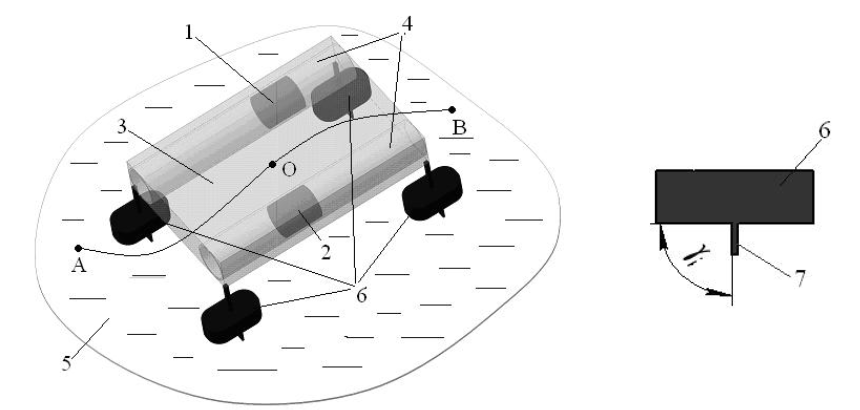
\includegraphics[width=0.7\linewidth]{JatsunRobot.png}%
	\caption{Схематичное изображение плавающего робота и схема поплавка}
	\label{JatsunRobot}
\end{figure}

В диссертации~\cite{Klenov_diss} рассмотрена локомоционная мобильная платформа, перемещающаяся в жидкости за счет изменения распределения масс (см. рисунок~\ref{TolikRobot}). Разработана математическая модель плоскопараллельного движения для идеальной жидкости и математическая модель движения с учетом внешних сил, действующих на объект со стороны жидкости. Изготовлен натурный образец~\cite{patent_BNR} и проведены экспериментальные исследования, при этом платформа движется по поверхности жидкости.

\begin{figure}[h]
	\centering
	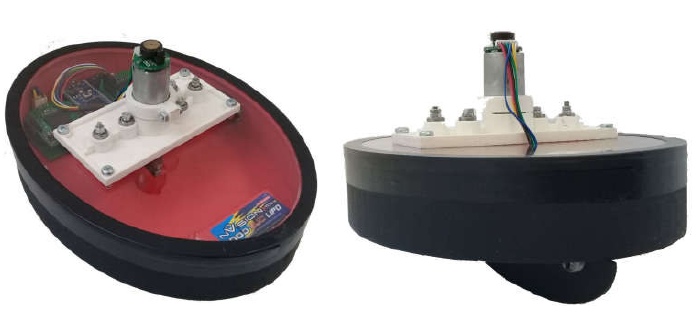
\includegraphics[width=0.7\linewidth]{TolikRobot.png}%
	\caption{Локомоционная мобильная платформа, перемещающаяся в жидкости за счет изменения распределения масс}
	\label{TolikRobot}
\end{figure}

В работе~\cite{Tallapragada_2015} рассмотрен водный робот, имеющий форму профиля крыла NACA 0030 (см. рисунок~\ref{TallapragadaRobot}). Робот перемещается в жидкости за счет периодического вращения внутреннего ротора. Разработана математическая модель движения, учитывающая сход вихрей с острой кромки. Проведены экспериментальные исследования. 

\begin{figure}[h]
	\centering
	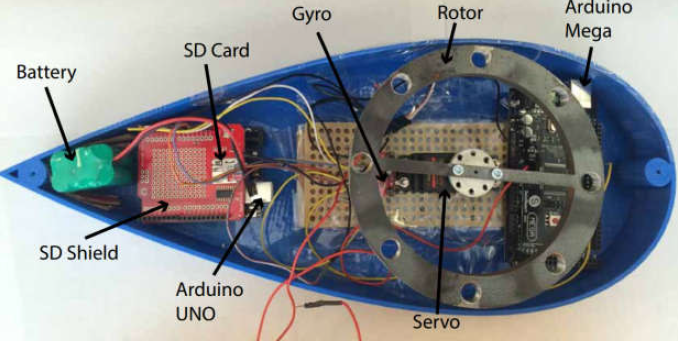
\includegraphics[width=0.7\linewidth]{TallapragadaRobot.png}%
	\caption{Водный робот, имеющий форму профиля крыла NACA 0030}
	\label{TallapragadaRobot}
\end{figure}

А в работе~\cite{Pollard_Tallapragada_2019} проведено сравнение маневренности вышеописанного робота при различных вариантах исполнения хвостовой части корпуса: полностью жесткий корпус, корпус со свободно вращающимся однозвенным хвостом, два варианта корпуса со свободно вращающимся двузвенным хвостом (см. рисунок~\ref{TallapragadaRobot2}).

\begin{figure}[h]
	\centering
	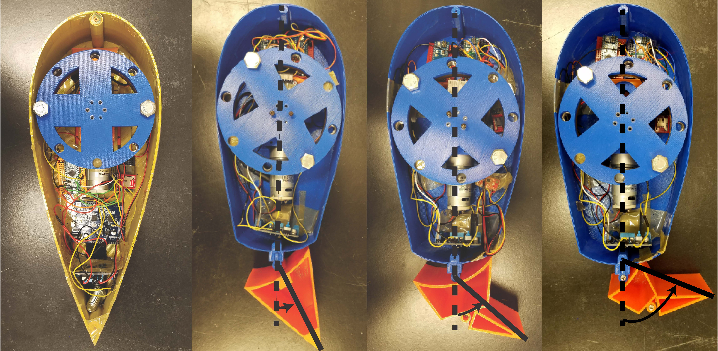
\includegraphics[width=0.7\linewidth]{TallapragadaRobot2.png}%
	\caption{Варианты исполнения водного робота со свободно вращающимся хвостом}
	\label{TallapragadaRobot2}
\end{figure}

В работе~\cite{Wang_Tan} рассмотрен рыбоподобный робот, перемещающийся за счет периодического движения хвостового плавника (см. рисунок~\ref{WangRobot}). Представлена модель движения, проведены экспериментальные исследования. Сделаны сравнения результатов моделирования и экспериментов.

\begin{figure}[h]
	\centering
	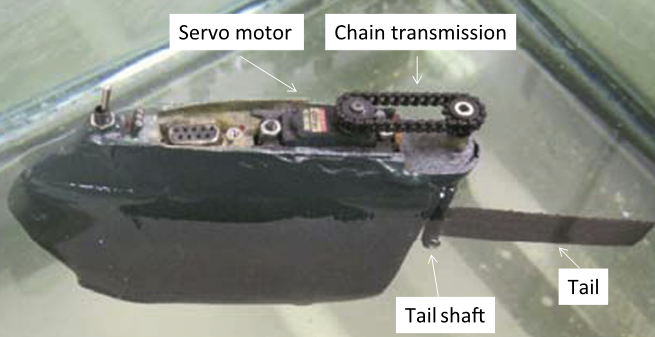
\includegraphics[width=0.7\linewidth]{WangRobot.png}%
	\caption{Рыбоподобный робот, перемещающийся за счет периодического движения хвостового плавника}
	\label{WangRobot}
\end{figure}

В работе \cite{Ramodanov_Tenenev} рассматривается задача о движении тела в вязкой жидкости, за счет перемещения внутренних масс, при котором внешняя оболочка тела остается неизменной. Приведена математическая модель, построенная на гидродинамических уравнениях Навье-Стокса. В результате численного моделирования показано существенное влияние сил и момента вязкого сопротивления на траекторию движения, выявлены отличия движения тела в вязкой жидкости по сравнению с идеальной. На основе полученных результатов в работе \cite{Vetchanin_Tenenev_2011} решена задача оптимального управления движением тела по заданной траектории за счет перемещения внутренних масс, с применением гибридного генетического алгоритма. В результате получены аппроксимационные зависимости для сил, действующих на тело.

Исследование характеристик движения тела с переменным распределением массы в трехмерной вязкой жидкости проведено в работе \cite{Vetchanin_Mamaev_Tenenev_ND_2012}, а в работе \cite{Kilin_Vetchanin_DAN_2016} рассмотрено управляемое движение при наличии циркуляции вокруг тела. В этих работах показана возможность перемещения тела в произвольном направлении, а также возможность преодоления силы тяжести телом с плавучестью близкой к нулевой.





